\documentclass[output=paper]{langsci/langscibook} 
\author{Kordula de Kuthy\affiliation{Universität Tübingen}}
\title{Information structure}

% \chapterDOI{} %will be filled in at production

%\epigram{Change epigram in chapters/03.tex or remove it there }
\abstract{Information structure as the hinge between sentence and
  discourse has been at the center of interest for linguists working
  in different areas such as semantics, syntax or prosody for several
  decades. A constraint-based grammar formalism such as HPSG encoding
  multiple levels of linguistic representation within the architecture
  of signs opens up the possibility to elegantly integrate such
  information about discourse properties. In this article, we discuss
  a number of approaches that have explored how to best integrate
  information structure as a separate level into the representation of
  signs. We discuss, which lexical and phrasal priciples have been
  implemented in these approaches and how they constrain the
  distribution of the various information structural
  features. Finally, we discuss how the various approaches are used to
  formulate theories about the interaction of syntax, prosody and
  information structure. In particular, we will see several cases
  where (word order) principles that used to be stipulated in syntax
  can now be formulated as an interaction of syntax and discourse
  properties.  }

\maketitle

\begin{document}
\label{chap-information-structure}



\section{Introduction} 


The \textit{information structure} of a sentence captures how the meaning
expressed by the sentence is integrated into the discourse.
The \textit{information structure} thus encodes which part of an
  utterance is informative in which way, in relation to a particular context.
A wide range of approaches exists with respect to the question what
should be regarded as the primitives of the information structure.

It is now commonly assumed that there are three basic dimension of
information structure that are encoded in natural languages and that
have been assumed as the basic primitives: (i) A distinction between
what is new information advancing the discourse (\emph{focus}) and
what is known, i.e., anchoring the sentence in existing (or
presupposed) knowledge or discourse (\emph{background}), (ii) A
distinction between what the utterance is about (\emph{topic},
\emph{theme}) and what the speaker has to say about it
(\emph{comment}, \emph{rheme}), and (iii) and a dimension referred to
as \textit{information status} where entities that have already been
mentioned in the discourse \textit{given} ares distinguished from those
that haven't been mentioned. (\emph{new}). For all three ways of
partitioning the information structure, we find approaches within the
HPSG framework.
Example (\ref{ex:info-struc}) illustrated, how one utterance in the context of a question can be
structured according to different partitionings of information
structure.
\begin{exe}
\ex\label{ex:info-struc}
\begin{xlist}
\exi{Q:}  What does Sarah drink?
\exi{A:}  \begin{tabular}[c]{|c|c|c|}
    \multicolumn{2}{c|}{\small\textsl{background}} &
                                                     \multicolumn{1}{c}{\small\textsl{focus}}\\\hline Sarah & drinks &
                                                                                                                      TEA.\\\hline
    \multicolumn{1}{c}{\small\textsl{topic}} & \multicolumn{2}{|c}{\small\textsl{comment}}\\
  \end{tabular}
\end{xlist}

\end{exe}

The focus/background division with focus as the part of an utterance
that is informative with respect to the discourse is one of the most
commonly adopted partitioning when studying information structure, and
thus many approaches within the HPSG architecture as well assume a
division into focus and background, such as the ones that will be discussed in this
article: \cite{EV96a}, \cite{deKuthy2002a}, \cite{Webelhuth2007a-u},
\cite{song-bender:2012}, \cite{Paggio2009a-u},
\cite{Bildhauer2008a}. Less common within the HPSG framework are
approaches that take topic, i.e. the material that an utterance is
about, as the central notion and assume topic and comment (or theme
and rheme) as the primitives of the information structure. Most
approaches discussed here assume that the background has one
designated (mostly referential) element functioning as the topic (or
link), among them are \cite{EV96a}, \cite{deKuthy2002a},
\cite{Paggio2009a-u}.

A third aspect of the information structure is captured under the
notion of information status with primitives such as new and
given. Here the discourse status of referential elements is of
interest, i.e. whether they can be linked to previously mentioned
items, i.e. whether they are (discourse) old or given, or whether they
haven't been mentioned before and are thus (discourse) new. The
representation of information status has received comparatively little
interest within the HPSG community, the approach by
\cite{DeKuthy.Meurers-11} is one of the few approaches that
explicitly integrate this dimension into their information structural
architecture.

The need to represent discourse properties in a grammar architecture
of signs results from the insight that in many, if not all, languages
the way utterances are realized via their syntactic structure,
morphological patterns and prosody very often interacts with discourse
requirements of these utterances. In other words, approaches dealing
with constraints on word order in a particular construction need to
encode that this particular word order is only grammatical given a
particular context, or a particular accent pattern has to be connected
to a particular discourse status of the accented elements.
Most of the approaches discussed here include deal with such interface
questions, and we therefore discuss the particular word order and
phonetic theories that have been implemented in sections \ref{sec:word-order}
and \ref{sec:prosody} in detail. As a starting point, however, we will first
discuss the various architectural designs that have been implemented in
order to be able to formulate the specific theories integrating
discourse constraints.

\section{Information structure in the architecture of signs}

Several ways of representing information structure within the
architecture of signs have been pursued as part of the HPSG framework:
one of the earliest approaches, which is similar to the idea of
F-marking as pursued in many syntax-based approaches to information
structure in generative grammar (such as
\cite{Jackendoff72a-u},\cite{Selkirk84a-u}), has been proposed by
\cite{Mandahar94a-u}. He assumes that all signs have an additional
appropriate feature \textsc{info"=struc} which takes as its value
objects of the sort \textit{info-type}. A sign can then be specified
for the subtypes of \textit{info-type} shown in
Figure~\ref{fig:manand-info-struc} as its informational marking.
\begin{figure}[htb!]
  \begin{center}
        \textit{
           \begin{forest}
             [info-type
                [focus]
                [background
                     [link]
                     [tail]
                ]
             ]
           \end{forest}}
    \caption{Type hierarchy under \textit{info-type} of \cite{Mandahar94a-u}}
    \label{fig:manand-info-struc}
  \end{center}
\end{figure}

The distribution of the \textsc{info"=struc} values in a sign is determined by
the \textit{Focus Inheritance Principle}, which enforces that in every
phrase, the \textsc{info"=struc} value of the mother subsumes the values
of the \textsc{info"=struc} of all of its daughters. The consequence of
this principle is that if one daughter in a phrase is in the focus and
the other one in the ground, then the mother's \textsc{info"=struc} value is the
smallest common super-type of both, namely \textit{info-type}.

There are two problematic aspects of such an architecture. Firstly, it
leads to a proliferation of syntactic markup of non-syntactic
properties, in particular once one considers the full range of
information structure notions, such as focus and focus projection,
multiple foci, and the marking of other discourse functions such as
topic. And secondly, the perspective of information structure as
resulting from an independent interpretation process of syntactic
markup does not support a view of syntax, information structure, and
intonation as directly interacting modules, a view that can be nicely
implemented in a multi-layer frameworks such as HPSG.
More common are thus approaches that encode the information structure
as a separate layer, i.e., a feature with its own structural
representation.

In the original setup of signs introduced in \cite{ps2}, the feature
\textsc{context} is introduced as part of \textit{local} objects as a
place to encode information relating to the pragmatic context (and
other pragmatic properties) of utterances. In \cite{EV96a} it is
argued that it would be most natural to also represent information
structural information as part of this \textsc{context}
feature. \cite{EV96a} thus introduce the feature \textsc{info"=struc}
as part of the the \textsc{context} and since they couch their
approach into \cite{vallduvi:92} information packaging account,
\textsc{info"=struc} is further divided into \textsc{focus} and
\textsc{ground}. All \textsc{info"=struc} features take entire signs as
their values. The complete specification is shown in
Figure~\ref{fig:e-v-info-struc}.

\begin{figure}[htb!]
  \begin{center}
        \leavevmode
    \begin{avm}
    [\tp{sign}\\
     synsem|local|context|info-struc & [focus & sign\\
                                        ground & [link & sign\\
                                                  tail & sign]
                                       ]
    ]     
    \end{avm}
    \caption{Information structure in \cite{EV96a}}
    \label{fig:e-v-info-struc}
  \end{center}
\end{figure}

Another approach locating the representation of information structure
with in the \textsc{context} feature is the one by
\cite{Paggio2009a-u} as part of a grammar for Danish. The
\textsc{infostr} feature \textsc{topic}, \textsc{focus} and
\textsc{bg} take as their values list of indices. Since
\cite{Paggio2009a-u} includes Minimal Recursion Semantics (MRS,
\citep{CFPS2005a}) as the semantic representation\footnote{A detailed
  discussion of the properties and principles of MRS as implemented in
  HPSG can be found in \crossrefchaptert{semantics}.}, these indices
can be structure shared with the argument indices of the semantic
relations collected on the \textsc{RELS} list of the content of a
sign. The basic setup is illustrated in
Figure~\ref{fig:paggio-infostr}.
\begin{figure}[htb]
  \centering
        \leavevmode
    \begin{avm}
    [\tp{sign}\\
     synsem|local|context|infostr & [focus & list-of-indices\\
                                     topic & list-fo-indices\\
                                     bg & list-of-indices]
    ]     
    \end{avm}
  \caption{Information structure in \cite{Paggio2009a-u}}
  \label{fig:paggio-infostr}
\end{figure}

Several approaches encode infostruc as part of the \textsc{content},
such as \cite{song2018} and \cite{song-bender:2012}. Since they also
use MRS as the semantic representation language, they enrich the
architecture of \textit{mrs} structures. The information structure
itself is encoded via a feature \textsc{icons} (Individual
Constraints), that is introduced parallel to \textsc{HCONS} (handle
constraints) as part of the \textsc{content}.

\begin{figure}[htb]
  \centering
    \begin{avm}
    [\tp{sign}\\
     synsem|local|content & [\tp{mrs}\\
                             hook & [\tp{hook}\\
                                     icons-key & info-str\\
                                      clause-key & event]\\
                             rels & diff-list\\
                             hcons & diff-list\\
                             icons & \XlstI{..., [\tp{info-str}\\
                                                 clause & individual\\
                                                 target & individual], ...}
                           ]
    ]     
    \end{avm}
  \caption{Information structure in \cite{song-bender:2012}}
\end{figure}

As pointed out by \cite{deKuthy2002a}, assuming that the information
structure is part of \textit{local} objects (which it is if it is part
of the \textsc{context} in HPSG as proposed by \cite{EV96a} or part of
the \textsc{content}) is problematic in connection with a trace-based
account of unbounded dependencies.  Traces should not contribute
anything to the information structure of a sentence.  If one wants to
develop an information structure approach which is independent of the
decision of which kind of UDC theory one assumes, the only options for
placing the information structure attribute are \textit{synsem}
objects or signs.


Information structure as part of \textit{synsem} objects would suggest
that it plays a role in syntactic selection. This possibility is
assumed in \cite{BC2011b}, and they thus represent \textsc{info"=struc}
as a feature appropriate for \textit{synsem} objects (their account
will be discussed in more detail in section \ref{sec:word-order}.  A
third possibility is argued for in \cite{deKuthy2002a} and
\cite{Bildhauer2008a}, namely that information structure should not be
part of \textit{synsem} objects. As a result, they encode information
structure again as an additional feature of signs (similar to
\cite{Mandahar94a-u} approach discussed above), but it is argued that
the appropriate values should be semantic representations.

In \cite{deKuthy2002a}, a tripartite partition of information
structure into focus, topic, and background is introduced. As to the
question what kinds of objects should be defined as the values of
these features, De Kuthy proposes the values of the
\textsc{info"=struc} features to be chunks of semantic information.  It
is argued that the semantic representation proposed in \cite{ps2} is
not appropriate for her purpose, because the semantic composition is
not done in parallel with the syntactic build-up of a phrase. Instead,
the Montague-style semantic representation for HPSG proposed in
\cite{Sailer2000a} is adopted, in which \textsc{content} values are
regarded as representations of a symbolic language with a
model-theoretic interpretation. As the semantic object language under
\textsc{content} the language Ty2 (cf., \cite{Gallin75a-u}) of
two-sorted type theory is chosen. The resulting feature architecture
is shown in Figure~\ref{fig:info-struc}.

\begin{figure}[htb!]
  \begin{center}
\leavevmode
    \begin{avm}
     [\tp{sign}\\
      phon & list\\
      synsem & synsem\\
      info-struc &
      [\tp{info-struc}\\
        focus & list-of-mes\\
        topic & list-of-mes
      ] 
     ]
    \end{avm}
    \caption{The structure of \textsc{info"=struc} in \cite{deKuthy2002a}}
    \label{fig:info-struc}
  \end{center}
\end{figure}
The information structure is
encoded in the attribute \textsc{info"=struc} that is appropriate for
signs and has the appropriate features \textsc{focus} and
\textsc{topic}, with lists of so-called meaningful expressions
(semantic terms, cf.  \cite{Sailer2000a}) as values.

\section{Information structure principles}
\label{sec:inf-principles}

The above sketched approaches all assume that signs contain some kind
of structural representation of information structure, with the
consequence that they need to introduce principles that constrain the
values of the information structural features. Most approaches thus
formulate two types of principles as part of their grammar fragment,
one set of principles on the lexical level tying information structure to word
level properties such as accents, and another set of principles on the
phrasal level determining the distribution of information structure
values between mother and daughters in a phrase.


\subsection{Instantiating information structure on the word level}
\label{sec:instant}

In the approach of \cite{EV96a} prosodic properties of
English, in particular accent placement, are tied to specific information
structural properties of words and phrases. On the word level, they
thus introduce two principles that instantiate the information
structure \textsc{focus} and \textsc{link} when the word has a
particular accent. The two principles are shown in
Figure~\ref{fig:engdahl-word-principle}.
\begin{figure}[htb]
  \centering
  \begin{tabular}{@{}l@{}l@{}l@{}}
    \textit{word}\ $\to$
    &&
   \begin{avm}
    @1 [
      phon|accent & A\\
         info-struc|focus & @1
      ]
   \end{avm} 
\\[2ex]
    \textit{word}\ $\to$
    &&
   \begin{avm}
    @1 [
      phon|accent & B\\
         info-struc|ground|link & @1
      ]
   \end{avm} 

    \end{tabular}
  
  \caption{Information structure of words}
  \label{fig:engdahl-word-principle}
\end{figure}
Words with an A accent always contribute focal information, i.e. the
entire sign is structure-shared with the \textsc{info"=struc|focus}
value, words carrying a B accent contribute link information, i.e. the
entire sign is structure-shared with the
\textsc{info"=struc|ground|link} value.

A similar set of word level principles is introduced in the approach
of \cite{deKuthy2002a}, where the information structure of utterance
in German is also tied to words carrying particular accent patterns.
The phonology of signs is altered as shown in Figure~\ref{fig:accent}
to include an \textsc{accent} attribute to encode whether a word
receives an accent or not, and whether it is a rising or a falling
accent in case it receives one.
\begin{figure}[htb!]
\vspace{1ex}
    \begin{center}
          \begin{tabular}{@{}l@{\hspace{2em}}l@{}}
    \begin{avm}
      [\tp{sign}\\
       phon & [phon-string \tpv{list}\\
               accent \tpv{accent}
              ]
      ]
    \end{avm}
&
\textit{  \begin{forest}
        [accent
            [unaccented]
            [accented
                  [rising-accent]
                  [falling-accent]
            ]
        ]
  \end{forest}}
\\
     \end{tabular}
\caption{Representing pitch accents}
    \label{fig:accent}
    \end{center}\unskip
\end{figure}

The information structure of words is defined through the principle
shown in Figure~\ref{fig:words} which assigns the semantic
contribution of the word to the focus or topic specification in the
information structure representation of that word, depending on the
type of accent the word receives.
\begin{figure}[htb!]
  \begin{center}
    \begin{tabular}{@{}l@{}l@{}l@{}}
    \textit{word}\ $\to$
    &&
    \begin{avm}[
      phon|accent & falling-accent\\
      ss|loc|cont|lf & @1\\
      info-struc & [focus & \XlstI{@1}\\
                    topic & \elst]
      ]
    \end{avm}\\
\\%   &$\vee$\; &
%   \begin{avm}
%     [
%      phon|accent & rising-accent\\
%      ss|loc|cont|lf & @1\\
%      info-struc &(  [focus & \elst\\
%                    topic & \XlstI{@1}]\\
%   $\vee$\; \\
%                   [focus & \XlstI{@1}\\
%                    topic & \elst])
%      ]
%   \end{avm}\\[2em]
    &$\vee$\; &
     \begin{avm}
     [
      phon|accent & unaccented\\
         info-struc & [focus & \elst\\
                    topic & \elst]
      ]
   \end{avm}\\\\
    &$\vee$\; &
    \ldots
    \end{tabular}
    \caption{Relating intonation and information structure}
    \label{fig:words}
   \end{center}\unskip
\end{figure}


\subsection{Information structure principles on the phrasal level}
\label{sec:infostruc-phrase}

\subsubsection{Information packaging \citep{EV96a}}

One of the first approaches integrating an explicit representation of
information structure into the HPSG architecture, \cite{EV96a} encode
the information structure as part of the \textsc{context} of signs
with the help of an additional feature \textsc{info"=struc}. As
discussed above, on the lexical level the instantiation of these
features can be triggered by phonetic properties, such as certain
accents, for intonation languages like English. Phrasal signs must
then satisfy the \textsc{info"=struc} instantiation constraints in
(\ref{ex:infostruc-instantiation}).
\begin{exe}
  \ex\label{ex:infostruc-instantiation} \textsc{info"=struc} \textit{instantiation principles for English:}
  \begin{xlist}
    \exi{} Either (i) if a \textsc{Daughter}'s \textsc{info"=struc} is instantiated, then the mother inherits this instantiation (for narrow foci, links and tails),
    \exi{} or (ii) if the most oblique \textsc{daughter}'s \textsc{focus} is instantiated, then the \textsc{focus} of the mother is the sign itself (wide focus).
  \end{xlist}
\end{exe}

As a result, the resulting structure including a wide VP focus with
the relevant \textsc{info"=struc} values is shown in
Figure~\ref{fig:info-packaging}.

\begin{figure}[htb]
  \centering\avmoptions{}
           \begin{forest}
             [ S{[fin]}\\
               \begin{avm}
                 \[info-struc \[focus \@3\\
                 ground\|link \@4\]\]
               \end{avm}
                [\idx{4}\\
                 NP{[nom]}\\
                \begin{avm}
                  \[phon\|accent B\\
                   info-struc\|ground\|link \@4\]
                \end{avm}
                 [{the president}]
                 ]
                [\idx{3}\\
                 VP{[fin]}\\
                \begin{avm}
                  \[info-struc\|focus \@3\]
                \end{avm}
                     [\idx{2}\\
                 VP{[fin]}\\
                \begin{avm}
                  \[phon\|accent u\]
                \end{avm}
                 [hates]]
                     [\idx{1}\\
                 NP{[acc]}\\
                \begin{avm}
                  \[phon\|accent A\\
                   info-struc\|focus \@1\]
                \end{avm}
                  [{the Delft China Set}]]
                ]
             ]
           \end{forest}  
  \caption{An example for VP focus in \cite{EV96a}}
  \label{fig:info-packaging}
\end{figure}

According to the principle in (\ref{ex:infostruc-instantiation}),
since the rightmost NP daughter carries an A accent, the entire sign
is structure-shared with the focus value (or, in Engdahl and Valluvi's
terms the focus value ``is instantiated''), the second clause of the
principle in (\ref{ex:infostruc-instantiation}) applies and the focus
value of the VP mother is the sign itself, which is then inherited by
the sentence itself.


\subsubsection{Information structure as structured meanings \citep{deKuthy2002a}}
\label{sec:struc-meaning}
The structured meaning approach
\citep{Stechow81a-u,Jacobs83a,Krifka92a-u-kopiert} provides a
compositional semantic mechanism based on separate representations of
the semantic contribution of the focus and that of the
background. \citet{deKuthy2002a} and \cite{Webelhuth2007a-u} worked
out how such a structured meaning approach can be integrated into the HPSG
architecture.

As discussed above, in \cite{deKuthy2002a}, the information structure
is encoded in the attribute \textsc{info"=struc} that is appropriate
for signs and has the appropriate features \textsc{focus} and
\textsc{topic}, with lists of so-called meaningful expressions as
values. The background of a sentence in De Kuthy's approach is then defined
to be that part of the logical form of the sentence which is neither
in focus nor in topic.  This characterization of background closely
resembles the definition of background employed by the so-called
\textit{structured meaning} approaches to focus of
\cite{Stechow81a-u}, \cite{Jacobs83a}, or \cite{Krifka92a-u-kopiert}.
The \textsc{info"=struc} value of a simple sentence with the focus as
indicated in \ref{ex:peter} is thus structured as shown in
Figure~\ref{fig:focus-backgr}.
\begin{figure}[htb!]
\begin{exe}
  \ex\label{ex:peter} \gll Peter {\LF}liest ein BUCH.{\RF}\\
           Peter {\hspaceThis{\LF}}reads a book\\
\end{exe}
  \begin{center}
    \begin{avm}
      [s|loc|cont|lf  $\exists x \[book'\(x\) \wedge read'\(p,x\)\]$\\
       info-struc  [focus & \XlstI{$\lambda y \exists x\[book'\(x\) \wedge read'\(y,x\)\]$}\\
                     topic & \elst]
      ]
    \end{avm}
    \caption{A sign representation including information structure}
    \label{fig:focus-backgr}
  \end{center}\unskip
\end{figure}

The information"=structure values of phrases are constrained by
principles such as the one in Figure~\ref{fig:focus-projection}.  The
simplest case are those sentences where the focus or the topic does
not project, i.e., only the words bearing an accent are in the topic
or in the focus of an utterance.
%
\begin{figure}[htb!]
\begin{center}
  \textit{phrase} $\to$ \begin{tabular}[t]{@{}l@{}l@{}}
    &
    \begin{avm}
      [
      info-str|focus  @1\ $\oplus$ \rel{collect-focus}\,(@2)\\
      head-dtr|info-str|focus @1\\
      non-head-dtrs @2 ]
    \end{avm}\\[5ex]
   $\vee$\; & \begin{avm}
      [phon|phon-str @1 $\oplus\,$ @2\\
       ss|loc [cat|head & noun $\vee\,$ prep\\
                 cont|lf & @3
                ]\\
       info-str|focus \XlstI{@3}\\
       \rel{any-dtr}\,([phon|phon-str & @2\\
                        ss|l|cont|lf & @4\\
                        info-str|focus & \XlstI{@4}])
      ] 
    \end{avm}\\\\
    $\vee$\;& \begin{avm}
      [synsem|loc [cat|head & verb\\
                 cont|lf & @3
                ]\\
       info-str|focus \XlstI{@3}\\
       non-head-dtrs  \XlstI{..,[synsem [fpp \tpv{plus}\\
                                          loc|cont|lf  @4]\\
                                  info-str|focus \XlstI{@4}],..}] 
    \end{avm}\\[8ex]
    $\vee$\; & \ldots
     \end{tabular}
     \caption{Extended focus projection principle}
  \label{fig:focus-projection}
   \end{center}\unskip
\end{figure}
In this case, the mother of a phrase just collects the focus values of
all her daughters as ensured by the principle in
Figure~\ref{fig:focus-projection}
\footnote{The presentation differs from that in
  \citet{deKuthy2002a}, it is the one from \cite{dKM2003a}. Definitions of the auxiliary relations:
\begin{center}\avmoptions{center}\smallAvmFonts
\begin{avm}
\begin{tabular}[t]{@{}l@{}}
\rel{any-dtr}\,\(\@{1}\) := \[head-dtr & \@{1}\].\\ 
\rel{any-dtr}\,\(\@{1}\) := \[non-head-dtrs &
\rel{element}\,\(\@{1}\)\].\\
\\ 
\rel{collect-focus}\,\(\,\elst\,\) := \elst.\\ 
\rel{collect-focus}\,\(\,\<\[info-struc\|focus & \<\@{1}\>\] \ \| \@{2}\>\,\) := \<\@{1} \| \rel{collect-focus}\,\(\,\@{2}\,\) \>.
\end{tabular}\end{avm}\end{center}\vspace{-2\baselineskip}}. 
A similar principle is needed to determine the \textsc{topic} value of
phrases.

For cases of so-called focus projection in NPs and PPs, it is assumed in \cite{deKuthy2002a}
that it is sufficient to express that the entire NP (or PP) can be
focused if the rightmost constituent in that NP (or PP) is focused, as
expressed by the second disjunct of the principle in Figure~\ref{fig:focus-projection}.
If focus projection is possible in a certain configuration then this
is always optional, therefore the focus projection principle for nouns
and prepositions is formulated as a disjunct. The second
disjunct of the principle in Figure~\ref{fig:focus-projection}
ensures that a phrase headed by a noun or a preposition can only be in
the focus (i.e., its entire logical form is token identical to its
focus value) if the daughter that contributes the rightmost part of
the phonology of the phrase is entirely focused itself. Again, a
similar principle needs to be provided for the \textsc{topic} value of
nominal and prepositional phrases.

For the verbal domain, the regularities are known to be influenced by
a variety of factors, such as the word order and lexical properties of
the verbal head \citep[cf., e.g., ][]{vSU86a}.  Since verbs
need to be able to lexically mark which of their arguments can project
focus when they are accented, \cite{dKM2003a} introduce the boolean-valued feature
\textsc{focus"=projection"=potential (fpp)} for objects of type
\textit{synsem}.  Figure~\ref{fig:fpp-lieben} shows the relevant part
of the lexical entry of the verb \textit{lieben} (love) which allows
projection from the object but not the subject:
\begin{figure}[htb!]

\begin{center}
  \begin{avm}
    [ phon|phon-str  \XlstI{\phonfont{lieben}}\\
    arg-s  \XlstI{[loc|cat|head [\tp{noun}\\case & nom]\\fpp
      \tpv{minus}],[loc|cat|head [\tp{noun}\\case & acc]\\fpp
      \tpv{plus}]} ]
  \end{avm}
\caption{The focus projection potential of \textit{lieben}}
\label{fig:fpp-lieben}
\end{center}\unskip
\end{figure}

The third disjunct of the principle in
Figure~\ref{fig:focus-projection} then specifies under which circumstances
focus can project in the verbal domain: a phrase headed by a verb can
only be in the focus (i.e., its entire logical form is token identical
to an element of its focus value) if the daughter that has the focus
projection potential (\textsc{fpp} \textit{plus}) is entirely focused
itself.


\subsubsection{Information structure inheritance in MRS}

As introduced above, in the MRS based approach of \cite{Paggio2009a-u} the
information structure is part of the \textsc{context}, consisting of
\textsc{focus}, \textsc{topic} and \textsc{background} features which
are structure shared with the respective \textsc{index} values of the
semantic representation of a phrase. \cite{Paggio2009a-u} connects the
distribution of information structure values to particular clausal
types and introduces new phrasal subtypes which constrain the
distribution of information structure in the respective phrase. One
example for such a new phrasal subtype is the
\textit{focus-inheritance} as defined in figure
\ref{fig:focus-inheritance}, which then has to be cross-classified
with every basic phrasal subtype (such as \textit{hd-comp, hd-spec,
  had-adj}, etc.) in order to constrain the distribution of focus
values across all phrasal subtypes.

\begin{figure}[htp]
  \centering
  \begin{avm}
    [\tp{focus-inheritance}\\
    synsem|loc|context & [focus & \XlstI{@2,@1}\\ 
                           bg & @3]\\
    hd|synsem|loc|context & [focus & @1\\
                              bg & @3]\\
   non-hd & [synsem|loc|context|focus & \XlstI{@2}\\
             accent & true]]
  \end{avm}
  \caption{focus-inheritance in Paggio (2009)}
  \label{fig:focus-inheritance}
\end{figure}

The principle in \ref{fig:focus-inheritance} ensures that the list of
focus values of the mother is the list of focus values of the head
daughter plus the focus value of the non-head daughter, in case it is
accented. Similar principles are defined for the inheritance of
background values, also depending on the accent status of the non-head
daughter. Paggio further assumes that each phrasal subtype has further
subtypes connecting it to one of the information structure inheritance
phrasal types. For examples, she assumes that there is a phrasal
subtype \textit{focus-hd-adj} that is a subtype both of
\textit{hd-adj} and of \textit{focus-inheritance}. Finally, clausal
types are introduced that account for the information structure values
at the top level of a clause. For example, the
\textit{decl-main-all-focus} as shown in figure
\ref{fig:decl-main-all-focus}, is a clause, in which both the
background and the topic values are empty and the mother collects the
focus values from the head and the non-head daughter.
\begin{figure}[htp]
  \centering
  \centering\avmoptions{}
           \begin{forest}
[
  \begin{avm}
    \[\tp{decl-main-all-focus}\\
       ctxt\|... & \[\tp{all-focus}\\
                   topic & \elst\\
                    focus & \XlstI{\@2,\@1}\\
                     bg & \elst\]
     \]
  \end{avm}
[
\begin{avm}
  \[ctxt\|...\|focus & \XlstI{\@1}\]
\end{avm}
]
[
\begin{avm}
  \[ctxt\|...\|focus & \@2\]
\end{avm}
]
]    
     \end{forest}
  \caption{Declarative all-focus construction}
  \label{fig:decl-main-all-focus}
\end{figure}


Different from Paggio's approach, \cite{song2018},
\cite{song-bender:2012} locate the representation of information
structure within the MRS based \textsc{content} value of signs. The
list elements of information structural values build up for a phrase
consists of focus, background or topic elements co-indexed with the
semantic \textsc{index} values of the daughters of that phrase.  The
main point of their approach is that they want to be able to represent
underspecified information structural values, since very often a
phrase, for example with a certain accent pattern, is ambiguous with
respect to the context in which it can occur and thus is ambiguous
with respect to its information structure values.  An example they
discuss is the one in (\ref{ex:underspec-focus}), where the first
sentence could be an answer to the question \textit{What barks?} and
thus signal narrow focus, whereas the second utterance could be answer
to the question \textit{What happened?} and signal broad focus.
\begin{exe}
  \ex\label{ex:underspec-focus}
  \begin{xlist}
    \ex {\LF The \textsc{dog}\RF} barks.
    \ex {\LF The \textsc{dog} barks\RF.}
  \end{xlist}
\end{exe}
The approach pursued in \cite{song-bender:2012} thus assumes, that the
two possible readings in (\ref{ex:underspec-focus}) are further
specializations of one MRS which is associated with one syntactic
structure and includes underspecified values, in particular the type
of the \textsc{icons} element for the constituent \textit{barks},
leaving it open whether it is part of the focus or not.  Unfortunately
they don't specify how a potential focus projection or focus
instantiation principle for a non-ambiguous phrase could look like in
their approach. They only mention that ``it at least plausible that
MRS and ICONS will contain enough information to calculate the range
of fully-specified information structures for each sentence''.

\section{Topics}
\label{sec:topic}

Most HPSG approaches are based on a focus/background division of the
information structure. To capture aspects of a topic vs. comment
distinction, or to be able to specify topics as a special element in
the background, they include an additional feature or substructure for
topics. \cite{EV96a}, for example, divide the \textsc{ground} into
\textsc{link} and \textsc{tail}, where the link is a special element
of the background linking it to the previous discourse, just like
topics. In the approaches of \cite{deKuthy2002a},
\cite{song-bender:2012}, \cite{Paggio2009a-u}, and additional feature
\textsc{topic} is introduced, parallel to \textsc{focus} and
\textsc{background}, in order to distinguish discourse referents as
topics from the rest of the background.

Most approaches don't introduce separate mechanisms for the
distribution of \textsc{topic} values, but assume that similar
principles as the ones introduced for focus can constrain topic
values, as mentioned above for the approach of \cite{deKuthy2002a}. A
more specific example can be found in \cite{Paggio2009a-u}, where a
constraint on topicalization constructions including a topic-comment
partitioning is formulated, as illustrated in
Figure~\ref{fig:inv-topic-comment}.
\begin{figure}[htb]
  \centering\avmoptions{}
           \begin{forest}
[
  \begin{avm}
    \[\tp{inv-topic-comment}\\
       ctxt\|... & \[\tp{topic-comment}\\
                   topic & \XlstI{\@1}\\
                    focus & \@2\\
                     bg & \XlstI{\@3,\@1}\]
     \]
  \end{avm}
[
\begin{avm}
  \[ctxt\|... & \[topic & \XlstI{\@1}\\
                  bg & \XlstI{\@1}\]\]
\end{avm}
]
[
\begin{avm}
  \[ctxt\|... & \[focus & \@2\\
                  bg & \@3 \]\]
\end{avm}
]
]    
     \end{forest}
  \caption{Topicalization construction with extracted topic}
  \label{fig:inv-topic-comment}
\end{figure}
This \textit{inv-topic-comment} phrasal type constrains the
information structure values of topicalization constructions in Danish
characterized by subject verb inversion, where the topic corresponds
to the topicalized complement, as illustrated by the example in
(\ref{ex:inv-topic-comment}) from \cite{Paggio2009a-u}.
\begin{exe}
  \ex\label{ex:inv-topic-comment}\gll
  og [ i det nederste vindue]$_{T}$ [ tager man og saetter urtepotten]$_F$\\
 and {} in the lowest window {} takes one and puts flowerpot.\textsc{def}\\
  \trans 'And in the lowest window you put the flowerpot.'
\end{exe}


\section{Givenness}
\label{sec:givenness}

In \cite{DeKuthy.Meurers-11}, it is shown how
the HPSG approach to information structure of \cite{deKuthy2002a} and
colleagues can be extended to capture givenness and to make the right
predictions for so-called \emph{deaccenting}, which has been shown to be
widespread \citep{buering:06}.  In contrast to
\cite{Schwarzschild99a-u}, who spells out his approach in the framework
of alternative semantics \cite{Rooth92a-u}, they show how the notion of
givenness can be couched in a standard structured meaning approach --
thereby preserving the explicit, compositional representations of focus.

The example in in (\ref{ex:vehicle-context}) illustrated the necessity
to include information about the givenness into information structural
setup.

\begin{exe}
  \ex\label{ex:vehicle-context} The conference participants are
  renting all kind of vehicles.  Yesterday, Bill came to the
  conference driving a red convertible and today he's arrived with a
  blue one. \begin{xlist} \ex\label{ex:vehicle-context-question} What did John rent?
    \ex\label{ex:green} He (only) rented {\LF}a \textsc{green}
    convertible{\RF}.
  \end{xlist}
\end{exe}


The context in (\ref{ex:vehicle-context}) introduces some conference participants, Bill, the rental of
vehicles, and red and blue convertibles into the discourse.  Based on
this context, when considering the question
(\ref{ex:vehicle-context-question}) asking for the object that John is
renting as the focus, one can  answer this question with sentence (\ref{ex:green}), where
\textit{a green convertible} is the focus: Out of all the things John
could have rented, he picked a green convertible. In this focus, only
\textit{green} is new to the discourse, whereas convertibles were
already given in the context, and still the entire NP is in the focus

To capture such cases of focus projection, an additional feature
\textsc{given} is introduced as part of the setup of
\cite{deKuthy2002a} as already discussed in section \ref{sec:struc-meaning}. The
relation between pitch accents and the information structure of words
is still defined by the principle shown in Figure~\ref{fig:words}
depending on the type of accent the word receives.
%
\avmoptions{active}%
\begin{figure}[htb!]
\begin{center}
    \textit{word}\quad $\to$\quad
\begin{avm}
    % \begin{tabular}{@{}l@{}l@{}l@{}}
    % &&
    [
      phon|accent & accented\\
      ss|loc|cont|lf & @1\\
      struc-meaning & [focus & \XlstI{@1}\\
%                       topic & \elst\\
                        given & \elst]
      ]
% \\
% \\%   &$\vee$\; &
%   \begin{avm}
%     [
%      phon|accent & rising-accent\\
%      ss|loc|cont|lf & @1\\
%      info-struc &(  [focus & \elst\\
%                    topic & \XlstI{@1}]\\
%   $\vee$\; \\
%                   [focus & \XlstI{@1}\\
%                    topic & \elst])
%      ]
%   \end{avm}\\[2em]
    \ $\vee$\; 

     [
      phon|accent & unaccented\\
         struc-meaning & [focus & \elst\\
%                       topic & \elst\\
                       given & \elst]
      ]
    \ $\vee$\; 
    \ldots
   \end{avm}
    \caption{Relating intonation and information structure for words}
    \label{fig:words}
   \end{center}\unskip
\end{figure}

We extend the Focus Projection Principle of
\citet{dKM2003a} with a disjunct capturing focus
projection in the presence of givenness. Figure~\ref{fig:verbal-focus-projection} shows the resulting principle.
% \footnote{The
%   auxiliary relations are defined
%   as:\vspace{-1.4ex}
% \begin{center}\avmoptions{center}\smallAvmFonts
% \begin{avm}
% \begin{tabular}{@{}l@{}}
% \begin{tabular}[t]{@{}l@{}}
% \rel{any-dtr}\,\(\@{1}\) := \[head-dtr & \@{1}\].\\ 
% \rel{any-dtr}\,\(\@{1}\) := \[non-head-dtrs &
% \rel{element}\,\(\@{1}\)\].\\
% \end{tabular}\\\rule{0em}{3.8ex}
% \begin{tabular}[t]{@{}l@{}}
% \rel{collect-focus}\,\(\,\elst\,\) := \elst.\\ 
% \rel{collect-focus}\,\(\,\<\[struc-meaning\|focus & \<\@{1}\>\] \ \| \@{2}\>\,\) := \<\@{1} \| \rel{collect-focus}\,\(\,\@{2}\,\) \>.
% \end{tabular}\end{tabular}\end{avm}\end{center}\vspace{-1.6\baselineskip}}
%
\begin{figure}[htb!]
\begin{center}
  \textit{phrase} $\to$ \begin{tabular}[t]{@{}l@{}}

    \begin{avm} \phantom{$\vee$\;}
      [
      struc-meaning|focus  @1\ $\oplus$ \rel{collect-focus}\,(@2)\\
      head-dtr|info-str|focus @1\\
      non-head-dtrs @2 ]
    \end{avm}\\[6ex]
   \begin{avm} $\vee$\; 
      [phon|phon-str @1 $\oplus\,$ @2\\
       ss|loc [cat|head & noun $\vee\,$ prep\\
                 cont|lf & @3
                ]\\
       struc-meaning|focus \XlstI{@3}\\
       \rel{any-dtr}\,([phon|phon-str & @2\\
                        ss|l|cont|lf & @4\\
                        struc-meaning|focus & \XlstI{@4}])
      ] 
    \end{avm}\\[16ex]
    \begin{avm} $\vee$\; 
      [synsem|loc [cat|head & verb\\
                 cont|lf & @3
                ]\\
       struc-meaning|focus \XlstI{@3}\\
       non-head-dtrs  \XlstI{..,[synsem [fpp \tpv{plus}\\
                                          loc|cont|lf  @4]\\
                                  struc-meaning|focus \XlstI{@4}],..}] 
    \end{avm}\\[14ex]
\begin{avm}  $\vee$\; 
      [ss|loc|cont|lf  @3\\
       struc-meaning|focus  \XlstI{@3}\\
       \rel{dtrs-list(\rel{given-sign-list} $\bigcirc$ 
                      <[ss|l|cont|lf & @4\\
                      struc-meaning & [focus & \XlstI{@4}]]> 
                      )}]
\end{avm}
     \end{tabular}
     \caption{Focus Projection Principle}
  \label{fig:verbal-focus-projection}
   \end{center}\unskip
\end{figure}
%



The fourth disjunct of the Focus Projection
Principle\footnote{The auxiliary relations are defined
  as:\vspace{-1.4ex}
\begin{center}\avmoptions{center}\smallAvmFonts
\begin{avm}
\begin{tabular}[c]{@{}l@{}}
\begin{tabular}[c]{@{}l@{}}
\rel{dtrs-list}\,\(\<\@{1}\|\@{2}\>\) := \[head-dtr & \@{1}\\ non-hd-dtrs & \@{2}\]
\end{tabular}\\\rule{0em}{7ex}
\begin{tabular}[c]{@{}l@{}}
\rel{given-sign-list} := \elst.\\
\rel{given-sign-list} := \<\[ss\|l\|cont\|lf & \@1\\
                          struc-meaning & \[given & \XlstI{\@1}\]\] \| \rel{given-sign-list}\>.\\
\end{tabular}\end{tabular}\end{avm}\end{center}\vspace{-1.6\baselineskip}} 
captures the previously unaccounted cases where given material in a
focused phrase is deaccented. Focus in those examples can project from a
focused daughter in a position which normally does not allow focus
projection.  This only is an option if all other daughters in that
focused phrase are \emph{given}.  Spelling this out, the fourth
disjunct of the principle in Figure~\ref{fig:verbal-focus-projection}
specifies that the mother of a phrase can be in the focus (i.e., the
entire \textsc{lf} value of the mother's \textsc{content} is token
identical to an element on the mother's \textsc{focus} list) if it is
the case that the list of all daughters (provided by \rel{dtrs-list})
consists of \textit{given} signs into which a single \textit{focused}
sign is shuffled ($\bigcirc$).\footnote{If only binary structures are
  assumed, as in the examples in this paper, the principle can be
  simplified. We here kept the general version with recursive
  relations following \citet{dKM2003a}, which also
  support flatter structures.} As before, a sign is focused if its
\textsc{lf} value is token identical to an element of its
\textsc{focus} value; and a sign is given if its \textsc{lf} value is
token identical to an element of its \textsc{given} value.

The pitch accent in this example is on the adjective \textit{green} so
that the principle in Figure \ref{fig:words} licenses structure
sharing of the adjective's content with its \textsc{focus} value. In
the context of the question (\ref{ex:vehicle-context-question}), the
entire NP \textit{a green convertible} of example (\ref{ex:green}) is
in the focus. In the phrase \textit{green convertible}, the clause
licensing focus projection in NPs does not apply since the adjective
\textit{green}, from which the focus has to project in this case, is
not the rightmost element of the phrase.  What does apply is the
fourth disjunct of the principle licensing focus projection in
connection with givenness. Since the noun \textit{convertible} is
given, the adjective \textit{green} is the only daughter in the phrase
that is not given and focus is allowed to project to the mother of the
phrase. In the phrase \textit{a green convertible}, focus projection is
again licensed via the clause for focus projection in noun phrases,
since the focused phrase \textit{green convertible} is the rightmost
daughter in that noun phrase.


\section{Information structure and word order}
\label{sec:word-order}
The explicit representation of information structure as part of signs
in HPSG opens up the possibility of providing explanations for
constraints previously stipulated in syntax, such as word order
constraints, by deriving the constraints from the nature of the
integration of a sentence into the discourse. Many of the approaches
discussed in the previous section employ the information structural
architecture exactly in this way and formulate principles linking word
order to discourse properties.

One first such approach is presented in \cite{EV96a}, where word order
constraint for Catalan are couched into the information structure set
up discussed in section \ref{sec:infostruc-phrase}. The basic
observation is that in Catalan the word order within the sentential
core is VOS and that every constituent within this sentential core is
interpreted as focal. If an argument of the main verb of a sentence is
to be interpreted as non-focal, it mus be clitic-dislocated. The
example in \ref{ex:catalan} from \cite{EV96a} illustrated such two
cases.

\begin{exe}
  \ex\label{ex:catalan}
  \begin{xlist}
    \ex\gll Ahir \LF {va tornar} a Barcelona el \textsc{president.} \RF\\
         yesterday return to Barcelona the president\\
   \ex\gll A Barcelona$_1$ \LF hi$_1$ {va tornar} el \textsc{president}.\RF\\
           to Barcelona  {} returned the president\\
   \ex \LF Hi$_1$ va tornar el \textsc{president}\RF a Barcelona.
\trans 'Yesterday, the president returned to Barcelona.'
  \end{xlist}
\end{exe}
 
With respect to modelling this within the HPSG account, they assume
that phrases associated with a \textsc{link} interpretation should be
constrained to be left dislocated whereas phrases associated with a
\textsc{tail} interpretation should be right attached.
They thus introduce the following ID schema for Catalan:
\begin{sloppy}
\begin{exe}
\ex  \textit{Head-Dislocation Schema for Catalan:}\\
  The \textsc{dtrs} value is an object of sort
  \textit{head-disloc"=struc} whose
  \textsc{head-dtr|""syn\-sem|""local|""category} value satisfies the
  description\\
  \begin{avm} [head \type{verb}[vform \type{finite}], subcat \elst]
  \end{avm}, and whose
  \textsc{disloc"=dtrs|""context|""info"=struc} value is instantiated and
  for each \textsc{disloc"=dtr}, the
  \textsc{head-dtr|""synsem|""local|""content} value contains an element
  which stands in a \textit{binding} relation to that
  \textsc{disloc"=dtr}.
\end{exe}
\end{sloppy}

The principle requires that the information structure value
dislocated daughters of a finite sentences has to be
\textsc{ground}. An additional LP statement then captures the relation
between the directionality of the dislocation and a further
restriction of the \textsc{ground} value, as illustrated in
Figure~\ref{fig:lp-catalan}.
\begin{figure}[htp]
  \centering
  \textsc{link} > \textsc{focus} > \textsc{tail}
  \caption{LP constraint on information structure in Catalan}
  \label{fig:lp-catalan}
\end{figure}
This LP statement is meant to ensure that link material must precede
focus material and focus material must precede tails. By this,
\cite{EV96a} want to ensure that left-detached constituents are always
interpreted as links and right-detached constituents as tails.

The insights from Engdahl and Vallduvi's approach are the basis for an
approach accounting for clitic left dislocation in Greek presented by
\cite{AK2002a}. The representation of information structure with the
features \textsc{focus}, and \textsc{ground} (further divided into
\textsc{link} and \textsc{tail}, is taken over as well as the
phonological constraints on words and the information"=structure
instantiation principle. In order to account for clitic left
dislocation, as illustrated in example \ref{ex:clld-greek}, an
additional feature \textsc{clitic} is introduced as appropriate for
\textit{nonlocal} objects.

\begin{exe}
  \ex\label{ex:clld-greek}
  \begin{xlist}
    \ex Pii simetehoun s' afti tin paragogi?
    \ex \gll Tin parastasi \textit{ti} skinothetise o Karolos \textsc{koun} ...\\
              the performance {} directed the Karolos Koun\\
  \end{xlist}

\end{exe}

The Linkhood Constraint shown in Figure~\ref{fig:clld-constraint}
ensures that links (i.e. elements whose \textsc{infostruc|link} value
is instantiated) can only be fillers that are ``duplicated'' in the
morphology by a pronominal affix, i.e. it is required that there is an
element on the \textsc{clitic} list of the head daughter.

\begin{figure}[htb]
  \centering
  \begin{avm}
    [\tp{clitic-left-disloc-phrase}\\
      info-struc|link & {@2}\\
      clitic & {\small @{$\sum_2$}}]
  \end{avm}
$\to$\ 
\begin{avm}
  @2[phon|accent & u\\
     head & @1], \textbf{H} [\tp{phrase}\\
                              head & verb\\
                              clitic & {@1} $\uplus$ @{$\sum_2$} ]
\end{avm}
  \caption{The Linkhood Constraint for clitic left dislocation phrases}
  \label{fig:clld-constraint}
\end{figure}

The Linkhood Constraint thus has two purposes, it ensures clitic
doubling and it connects the particular word order of left dislocated
phrase to discourse properties by requiring the filler daughter to be
the link of the entire clause.

The approach of \cite{deKuthy2002a} relates
the occurrence of discontinuous NPs in German to specific
information"=structural contexts, and \citet{dKM2003a}
show that the realization of subjects as part of fronted non-finite
constituent and its constraints can be accounted for based on
independent information"=structure conditions.

Based on the setup discussed in section \ref{sec:struc-meaning} above,
constraints are formulated that constrain the occurrence of
discontinuous NPs and fronted VPs based on their information structure
properties. The type of discontinuous NPs that are at the center of De
Kuthy's approach are so-called NP-PP split construction, in which a PP
occurs separate from its nominal head, as exemplified in
(\ref{ex:np-pp}).

Example (\ref{ex:np-pp}) illustrated the type of discontinuous NPs 
\begin{exe}
  \ex\label{ex:np-pp} \begin{xlist}
    \ex\label{ex:simple-fronted-pp}\gll \textsl{Über Syntax} hat Max sich [ein
 Buch] ausgeliehen.\\
         {about syntax} has Max self { a} book borrowed\\
       \trans 'Max borrowed a book on syntax.'
    \ex\label{ex:simple-fronted-np}\gll [Ein Buch] hat Max sich \textsl{über Syntax}    ausgeliehen.\\
 { a} book has Max self {about syntax} borrowed\\
\end{xlist}
\end{exe}

The information structure propertied of discontinuous noun phrases are
summarized in \cite{deKuthy2002a} in the following principle:
\begin{quote}
  In an utterance, in which a PP occurs separate from an NP, either
  the PP or the NP must be in the focus or in the topic of the
  utterance, but they cannot both be part of the topic or the same
  focus projection.
\end{quote}

The last restriction can be formalized as: they cannot be part of the
same meaningful-expression on the FOCUS list or the TOPIC list of the
\textsc{info"=struc} value of the utterance.

As discussed in \cite{dKM2003a}, it has been observed
that in German it is possible for ergative  and unergative verbs to realize a subject
as part of a fronted non-finite verbal constituent. This is
exemplified in (\ref{ex:erg-subj-fronted}).

\begin{exe}
\ex\label{ex:erg-subj-fronted}
  \begin{xlist}
  \ex\label{ex:erg-subj-fronted-indef}\gll [Ein Fehler unterlaufen] ist meinem Lehrer noch nie.\\
         {\LB}an$_{nom}$ error {crept in} is my teacher still never\\
         \trans 'So far my teacher has never made a mistake.'
  \ex\gll [Haare wachsen] können ihm nicht mehr.\\
          {\LB}hair$_{nom}$ grow can him not anymore\\
          \trans 'His hair cannot grow anymore.'
\ex\label{ex:nonerg-subj-fronted}
      \gll [Ein Außenseiter gewonnen] hat hier noch nie.\\
           {\LB}an$_{nom}$ outsider won has hier still never\\
        \trans 'An outsider has never won here yet.'
  \end{xlist}
\end{exe}

In order to account for the context-sensitive occurrence of such
fronted verbal constituents, specific information structure properties
of fronted verb phrases need to be expressed in a principle expressing
what De Kuthy and Meurers refer to as Webelhuth's generalization: In
an utterance in which a verb phrase occurs as a fronted constituent
(i.e., the filler of a head-filler phrase) this entire verb phrase
must be in the focus of the utterance (i.e., the \textsc{focus} value
of the fronted constituent must be identical to its semantic
representation).  Figure~\ref{fig:webelhuths-generalization} shows the
formalization of this principle.

%\textbf{Webelhuth's generalization:} In an utterance with a fronted
%verbal constituent, the entire fronted verb phrase must be in the focus
%of the utterance (nothing more, nothing less).

%\bigskip
%\textbf{Formalization:}
\begin{figure}[htb!]
\bigskip
\begin{flushleft}
\qquad\begin{avm}
  [\tp{head-filler-phrase}\\
  non-head-dtr|synsem|loc|cat|head & verb]
\end{avm}
$\to$\ 
\end{flushleft}
\begin{flushright}
\begin{avm}
  [info-struc|focus <@1>\\
  non-head-dtr  [info-struc|focus & <@1>\\
  synsem|loc|cont|lf & @1]]\qquad
\end{avm}\medskip
\caption{Webelhuth's generalization}
\label{fig:webelhuths-generalization}
\end{flushright}\unskip
\end{figure}  

Combining the new lexical specifications, the focus projection rule
for the verbal domain, and the partial fronting focus requirement with
the basic setup of \cite{deKuthy2002a} one obtains a theory which
predicts that subjects can only be part of a fronted verbal projection
if they can be the focus exponent. The sketch of an analysis for an
example such as (\ref{ex:noner-subj-fronted}) is illustrated in
Figure~\ref{fig:focus-exponent}.
  \begin{figure}[htb]
    \centering
    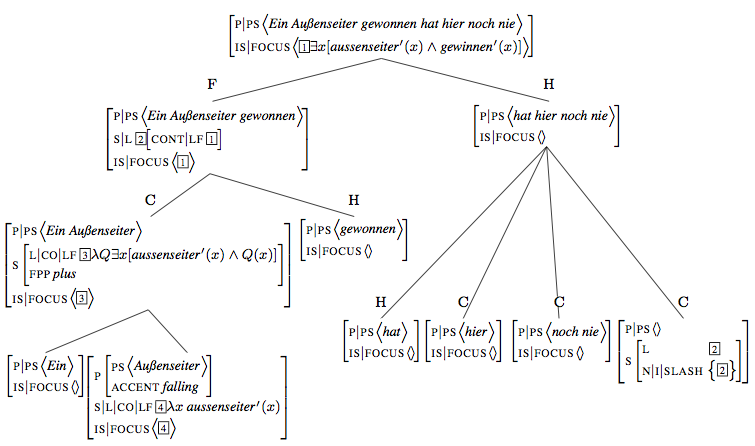
\includegraphics[scale=0.9]{figures/vp-focus-exponent}
    \caption{Partial VP fronting in \cite{dKM2003a}}
    \label{fig:focus-exponent}
  \end{figure}
  The entry of \textit{gewinnen} (to win) (the base form of the verb
  \textit{gewonnen} in example (\ref{ex:nonerg-subj-fronted}) in
  figure \ref{fig:lex-entry} encodes the lexical property that the
  subject of this intransitive verb has focus projection potential.
\begin{figure}[htb!]
\avmoptions{center,active}%
\begin{center}
  \begin{avm}
    [ phon & \XlstI{\phonfont{gewinnen}}\\
    arg-s & \XlstI{[fpp  \tpv{plus}\\
      loc|cat|head|case \tpv{nom}]} ]
  \end{avm}
\caption{The lexical entry of \textit{gewinnen} (to win)}
\label{fig:lex-entry}
\end{center}\unskip
\end{figure}

Under the assumption that in example (\ref{ex:nonerg-subj-fronted}) the
noun \textit{Außenseiter} carries a pitch accent, the
information"=structure principle for words in Figure~\ref{fig:words} ensures that the noun
contributes its \textsc{logical-form} value to its \textsc{focus}
value. The focus projection principle of
Figure~\ref{fig:focus-projection} ensures that the focus can
project over the entire NP \textit{ein Außenseiter}, i.e., its
\textsc{focus} element is identical to its \textsc{lf} value. Since
\textit{ein Außenseiter} as the subject of \textit{gewonnen} in the
tree in Figure~\ref{fig:focus-exponent} is lexically marked as
\textsc{fpp} \textit{plus}, the principle governing focus projection
in the verbal domain in Figure~\ref{fig:focus-projection}
licenses the focus to project over the entire fronted verbal
projection \textit{ein Außenseiter gewonnen}. The fronted constituent
thus contributes its \textsc{lf} value to its \textsc{focus} value. In
this example, the focus does not project further so that in the
head-filler phrase the focus values of the two daughters are simply
collected as licensed by the first disjunct of the focus principle in
Figure~\ref{fig:verbal-projection}. As a result, the
\textsc{focus} value of the fronted verbal projection is the
\textsc{focus} value of the entire sentence. Finally, note that the
example satisfies Webelhuth's generalization, which requires a fronted
verbal projection to be the focus of the utterance as formalized in
Figure~\ref{fig:webelhuths-generalization}.

In the same spirit, \cite{BC2010a} show that sentences in which
multiple elements have been fronted are directly linked to specific
types of information structure. In German as a V2 language, normally
exactly one constituent occurs in the position before the finite verb
in declarative sentences. But so-called multiple fronting examples
with more than one constituent occurring before the finite verb have
been well attested in naturally occurring data, two examples from
\cite{BC2010a} are shown in (\ref{ex:multiple-fronting}).
\begin{exe}
  \ex\label{ex:multiple-fronting}
  \begin{xlist}
    \ex\gll [Dem Saft] [eine kräftige Farbe] geben Blutorangen.\\
             to.the juice a more.vivid colour give blood.oranges\\
      \trans 'What give the jiuce a more vivid colour is blood oranges.'
    \ex\gll [Stets] [einen Lacher] [auf ihrer Seite] hatte die Bubi Ernesto Familie.\\
            always a laugh on their side had the Bubi Ernesto Family\\
        \trans 'Always good for a laugh was the Bubi Ernesto Family.'
  \end{xlist}

\end{exe}

But, as discussed by Bildhauer and Cook, such multiple fronting
examples seem to require very special discourse conditions in order to
be acceptable. Just like the fronted verb phrases discussed in
\cite{dKM2003a} above, \cite{BC2010a} propose
to analyze multiple fronting constructions in German as head-filler
phrases, which in this case introduce a topic shift. Following the
approach by \cite{Mueller2005d-unlinked}, multiple fronting
configurations can be identified via the filler daughter which must
have a \textsc{head|dsl} (double shlash) value of type
\textit{local}. As introduced above, \cite{BC2010a} assume that an
information structure attribute is specified in \textit{symsem}
objects, with the features \textsc{focus} and \textsc{topic} taking
lists of \textit{elementary predications} as their values. In general,
multiple fronting \textit{head-filler} phrases are restricted by the
constraint in \ref{fig:multiplefronting}.
\begin{figure}[htp]
  \centering
    \begin{avm}
      [\tp{head-filler-phrase}\\
      non-head-dtrs & \XlstI{[head|dsl & local]}]
    \end{avm}
$\to$\ 
  \begin{avm}
    [is & pres $\vee$ a-top-com $\vee$ ...]
  \end{avm}

\bigskip
    \begin{avm}
      [\tp{head-filler-phrase}\\
        is & pres]
    \end{avm}
$\to$\ 
  \begin{avm}
    [ss|loc|cat|head|dt & \XlstI{[loc|cont|rels @1]}\\
      hd-dtr|ss|is|focus & \XlstI{@1}]
  \end{avm}
  \caption{Relating multiple fronting to focus}
  \label{fig:multiplefronting}
\end{figure}

The first constraint ensures that \textit{head-filler} phrases that
are instances of multiple frontings are restricted to have an
\textit{is}-value of an appropriate type\footnote{\cite{BC2010a}
  assume that the type \textit{is} as the appropriate value for
  \textsc{is} has several subtypes specifying specific combinations of
  \textsc{topic} and \textsc{focus} values, such as \textit{pres} for
  presentational focus or \textit{a-top-com} for
  assessed-topic-comment.} The second constraint then ensures that in
presentational multiple frontings the designated topic of the non-head
daughter (i.e. the verbal head of the \textit{head-filler} phrase)
must be focused. The feature \textsc{dt} lexically specifies which
element, if any, is normally realized as the Topic for a particular
verb. This constraint thus encoded what \cite{BC2010a} call ``topic
shift'': the non-fronted element in a multiple fronting construction
that would preferably be the topic is realized as a focus. A similar
constraint is introduced for another instance of multiple frontings,
which is called \textit{propositional assessment} multiple
frontings. Here it has to be ensured that the designated topic must be
realized as the topic somewhere in the head-daughter and the
head-daughter must also contain a focused element.

\cite{Webelhuth2007a-u} provides another account of the special
information structural requirements of fronted constituents, in this
case of predicate fronting in English that is based on the interaction
of word order and information structural constraints.
\begin{exe}
  \ex I was sure that Fido would bark and \textit{bark he did}.
\end{exe}

The principles part of Webelhuth's account require that in such cases
of predicate fronting the auxiliary is focussed and the remainder of
the sentence is in the background. The interaction of the two
principles in Figure~\ref{fig:predicatepreposing}.
\begin{figure}[htb]
  \centering
  \begin{avm}
    [\tp{aux-wd}\\
      arg-s & \XlstI{NP, gap-ss}]
  \end{avm}
$\to$\ 
\begin{avm}
  [ss|status & foc\\
   arg-s & \XlstI{[status & bg], gap-ss}]
\end{avm}

\bigskip
\begin{avm}
  [\textit{pred-prepos-ph}]
$\to$\ 
\begin{avm}
  [\textit{hd-fill-ph}\\
    non-hd-dtr & [ss|status & bg]]
\end{avm}
  
\end{avm}
  \caption{Predicate preposing phrases}
  \label{fig:predicatepreposing}
\end{figure}
The first constraint ensure that auxiliary words whose predicate
complement could be preposed (i.e. is of type \textit{gap-ss} have the
information status \textit{focus}, whereas the status of the first
argument (the subject) is \textit{background}. Additional constraints
then ensure that auxiliary words with a gapped second argument can
only occur in predicate preposing phrases, and vice versa, that
predicate preposing phrases contain the right kind of auxiliary.

\section{Information structure and prosody}
\label{sec:prosody}
A lot of languages mark information structure prosodically, as for
example English and German, where pitch accents of various shapes are
used to mark focus. Accordingly, several of the above discussed
approaches include a component, which enriches the phonology representation
of signs such that is allows the integration of the necessary prosodic
aspects, as for example accents.

\cite{EV96a} assume, that signs can be marked for particular accents
signalling focus or links in English, so-called A and B accents.  In a
similar way, \cite{deKuthy2002a} extend the \textsc{phon} value such
that it includes a feature \textsc{accent}, in order to formulate
constraints on the connection between accents and information
structure markings.  Since most of the above discussed approaches
don't include a detailed analysis of the prosodic properties of the
respective language that investigated with respect to discourse
properties, most approaches don't go beyond the postulation of one or
two particular accents, that are somehow encoded as part of the
\textsc{phon} value. These accents then more or less serve as an
illustration how lexical principles can be formulated within a
particular theory that constrain the distribution of information
structural values on the lexical level. The more articulate such a
representation of \textsc{phon} values including accent pattern,
intonation contours, boundary tone etc is, the more detailed the principles
could be that are needed to connect information structure to
prosodic patterns in languages that signal discourse properties via
intonation contours.

In \cite{Bildhauer2008a} such a detailed account of the prosodic
properties of Spanish is developed together with a proposal how to
integrate prosodic aspects into the \textsc{phon} value, also allowing
a direct linking of the interaction of prosody and information
structure.  In his account, the representation of \textsc{phon} values
in HPSG is enriched to include four levels of prosodic constituency,
i.e., phonological utterance, intonational phrases, phonological
phrases and prosodic words. The lowest level, prosodic words of type
\textit{pwrd}, include the features \textsc{segs}, which correspond to
the original \textsc{phon} value assumed in HPSG, and additional
features such as \textsc{pa} for pith accents or \textsc{bd} for
boundary tones, to encode whether a boundary tone is realized on that
word. The additional features \textsc{ut} (phonological utterance),
\textsc{ip} (intonational phrase) and \textsc{php} (phonological phrase)
encode via the the typ \textsc{epr} (edges and prominence) which role
a prosodic word plays in higher level constituents. For examples, the
feature \textsc{dte} (designated terminal element) specifies, whether
the word is the most prominent in a phonological phrase. A sign's
\textsc{phon} list then contains all \textit{pwrd} objects and
relational constraints define the roles each prosodic word plays in
the higher prosodic constituents. This flat representation of prosodic
constituency still allows to express constraints about intonational
contours associated with certain utterance types. One example
discussed in Bildhauer's work is the contour associated with broad
focus declaratives in Spanish, which can be decomposed into a
sequence of late-rise (L*H) prenuclear accents, followed by an
early-rise nuclear accent (LH*), followed by a low boundary tone
(L\%). The constraint introduced to model this contour for declarative
utterances thus instantiates the \textsc{bd} value (boundary tone) of
the last \textsc{pwrd} in the \textsc{phon} list to low, instantiates
a nuclear pitch accent \textit{low-hig-star} on this rightmost
prosodic word and ensures that the a prenuclear pitch accent
\textit{low-star-high} is instantiated on every preceding compatible
prosodic word. The resulting constraint is shown in
Figure~\ref{fig:spanish-intonation}.

\begin{figure}[htp]
%  \centering
  \begin{tabular}[t]{l@{  }r@{}l@{}}
  \begin{avm}
    \textit{decl-tune(@1)}\end{avm} & $\leftrightarrow$ & \begin{avm} @1 = @2 $\oplus$ \<[pa & low-high-star\\
                                                                  bd & low]\> \end{avm}
$\wedge$\\
& &
\begin{avm}
  @2 = list([bd & none])
\end{avm}
$\wedge$\\
& &
\begin{avm}
@2 = list([pa & none]) $\shuffle$ list([pa & low-star-high])\end{avm}
\\[4ex]
\begin{avm}
[\textit{sign}\\
  embed & -]\end{avm} & $\rightarrow$ & \begin{avm} [phon @1] $\wedge$ decl-tune(@1)
  \end{avm}  \\
  \end{tabular}
  \caption{Intonational contour of Spanish declarative utterances}
\label{fig:spanish-intonation}
\end{figure}
% \section*{Abbreviations}
% \section*{Acknowledgements}

The second constraint in Figure~\ref{fig:spanish-intonation} ensure
that only unembedded utterances can be constrained to the just
described declarative tune. That this specific contour is then
compatible with a broad focus reading is ensured by an additional
principle expressing a general focus prominence constraint for
Spanish, namely that focus prominence has to fall on the last prosodic
word in the phonological focus domain, which in the case of a broad
focus can be the entire utterance. Figure~\ref{fig:focus-prominence}
shows the resulting principle in Bildhauer's account.
\begin{figure}[htp]
  \centering
  \begin{avm}
    [\tp{sign}\\
       cont & @1\\
       foc & @1]
$\rightarrow$\
[phon list $\oplus$ <[ut|dte & +]>]
  \end{avm}
  \caption{Focus Prominence in Spanish}
  \label{fig:focus-prominence}
\end{figure}
Since only words
that are the designated terminal element (\textsc{dte}) can bear a
pitch accent, the interplay of the two above principles ensures, that
in utterances with a declarative contour the entire phrase can be in
the focus. These principles thus nicely illustrate, how not only
lexical elements can contribute to the information structure via their
prosodic properties, but how entire phrases with specific prosodic
properties can be constrained to have specific information structural
properties.

\section{Conclusion}
\label{sec:conclusion}

We have discussed various possibilities of how to represent
information structure within the HPSG's sign-based architecture.
Several approaches from the HPSG literature were presented which all
have in common that they introduce a separate feature
\textsc{info"=struc} into the HPSG setup, but they differ in (i) where
they locate such a feature, (ii) what the appropriate values are for
the representation information structure, and (iii) how they encode
principles constraining the distribution and interaction of
information structure with other levels of the grammatical
architecture. Finally, we discussed a number of theories in which
phenomena such as word order are constrained to be only well-formed in
case they exhibit specific information structural properties.

%  {\sloppy
%  \printbibliography[heading=subbibliography,notkeyword=this] }


\printbibliography[heading=subbibliography,notkeyword=this] 
\end{document}
